    Comparing with \eqref{eq:conic_simp_temp_parab},
\begin{align}
	\label{eq:chapters/11/11/2/1/eqV}
	\vec{V} = \myvec{ 0 & 0 \\ 0 & 1},\
	\eta = -12
\end{align}
					From \appref{app:std-prm-P}, this corresponds to a standard parabola.  \begin{enumerate}
\item  Substituting the above values in 
					\eqref{eq:F-ell-hyp-parab},
the focus 
\begin{align}
	\vec{F} = .
\end{align}
\item 
					From \eqref{eq:dx-parab}
the directrix is given by
\begin{align}
\myvec{1 & 0}\vec{x} &= -3
\end{align}
\item The axis is the $x$-axis.
	\iffalse
\begin{align}
	\label{eq:chapters/11/11/2/1/eqAxis}
	\vec{m}^\top\brak{\vec{x}-\vec{F}} &= 0
\end{align}
where $\vec{m}$ is the normal vector to the axis and also the slope of the directrix.
\begin{align}
	\because \vec{n} = \myvec{1 \\ 0 }, \vec{m} &= \myvec{0 \\ 1} \\
	\eqref{eq:chapters/11/11/2/1/eqAxis} \implies \myvec{0 & 1}\myvec{\vec{x} - \myvec{3 \\ 0}} &= 0\\
	\text{or, }	\myvec{0 & 1}\vec{x} &= 0 
\end{align}
\fi
\item The latus rectum of a parabola is given by 
\begin{align}
	l &= \frac{\eta}{\lambda_2}  
	 = \frac{2\vec{u}^\top\vec{p_1}}{\lambda_2} \\
	 &= \frac{2\myvec{6 & 0}\myvec{1 \\ 0}}{1} \\
	 &= 12 \text{ units }
\end{align}
The relevant diagram is shown in Fig. \ref{fig:11/11/2/1Fig1}
\begin{figure}[!h]
	\begin{center}
		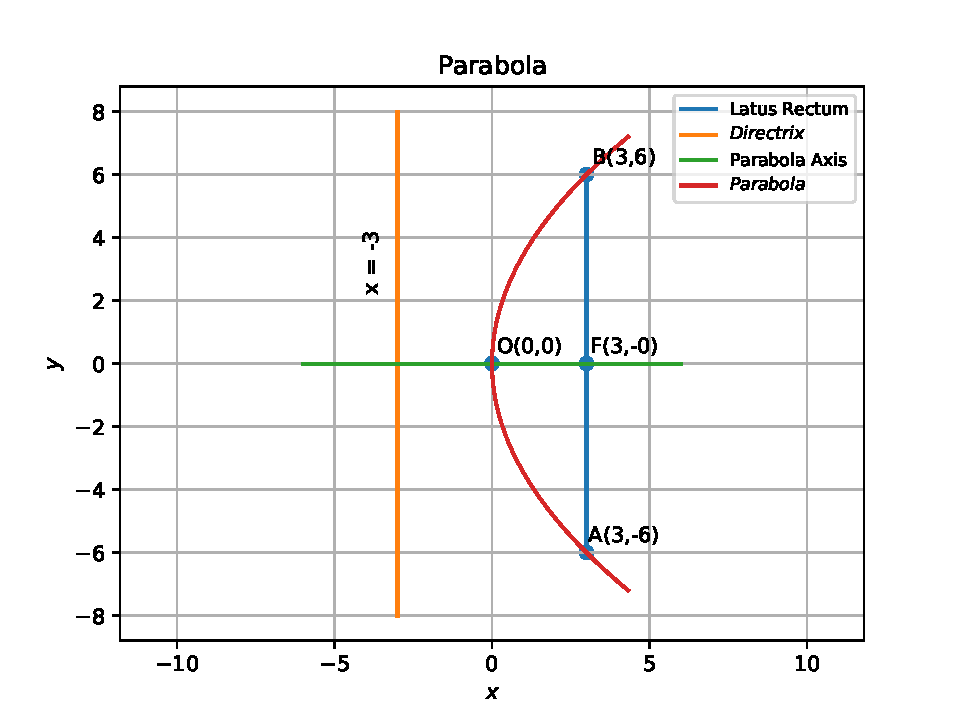
\includegraphics[width=\columnwidth]{chapters/11/11/2/1/figs/problem1.pdf}
	\end{center}
\caption{}
\label{fig:11/11/2/1Fig1}
\end{figure}
\end{enumerate}
